\documentclass[border=2pt,tikz]{standalone}
\usepackage[T1]{fontenc}
\usepackage{tikz}
\usetikzlibrary{positioning, arrows.meta, calc, fit, backgrounds, decorations.pathreplacing, shapes.geometric}

\definecolor{inputcol}{rgb}{0.17, 0.48, 0.71}
\definecolor{hiddencol}{rgb}{1.00, 0.50, 0.06}
\definecolor{outputcol}{rgb}{0.84, 0.15, 0.16}
\definecolor{frozencol}{rgb}{0.17, 0.63, 0.17}
\definecolor{ensemblecol}{rgb}{0.00, 0.75, 1.00}
\definecolor{residualcol}{rgb}{0.74, 0.74, 0.13}
\definecolor{directcol}{rgb}{0.55, 0.22, 0.08}
\definecolor{learnedcol}{rgb}{0.12, 0.30, 0.60}

\tikzset{
  ionode/.style={circle, draw, minimum size=6.5mm, inner sep=0pt,
                 font=\scriptsize, line width=0.45pt},
  input node/.style={ionode, fill=inputcol!20, draw=inputcol!70},
  output node/.style={ionode, fill=outputcol!20, draw=outputcol!70},
  tensor/.style={rectangle, draw, rounded corners=2pt,
                 minimum width=12mm, minimum height=25mm,
                 inner sep=3pt, font=\scriptsize, align=center,
                 line width=0.6pt},
  hidden block/.style={tensor, fill=hiddencol!15, draw=hiddencol!70},
  frozen block/.style={tensor, fill=frozencol!12, draw=frozencol!60},
  sum node/.style={circle, draw, minimum size=7mm, inner sep=0pt,
                   font=\normalsize, line width=0.5pt},
  avg node/.style={circle, draw, minimum size=7mm, inner sep=0pt,
                   font=\scriptsize, line width=0.5pt,
                   fill=ensemblecol!12},
  dots node/.style={font=\Large, inner sep=0pt},
  annot/.style={font=\scriptsize, text=black!65},
  lbl/.style={font=\scriptsize\bfseries,
              text=black!80, align=center},
  arr/.style={-{Stealth[length=2.5pt]}, line width=0.55pt, black!50},
  random arr/.style={arr, densely dashed, frozencol!70},
  learned arr/.style={arr, line width=0.9pt, learnedcol},
  direct arr/.style={-{Stealth[length=3pt]}, line width=0.7pt,
                     directcol, densely dotted},
  resbox/.style={draw=residualcol!55, dashed, rounded corners=3pt,
                 fill=residualcol!6, line width=0.55pt},
}

\begin{document}
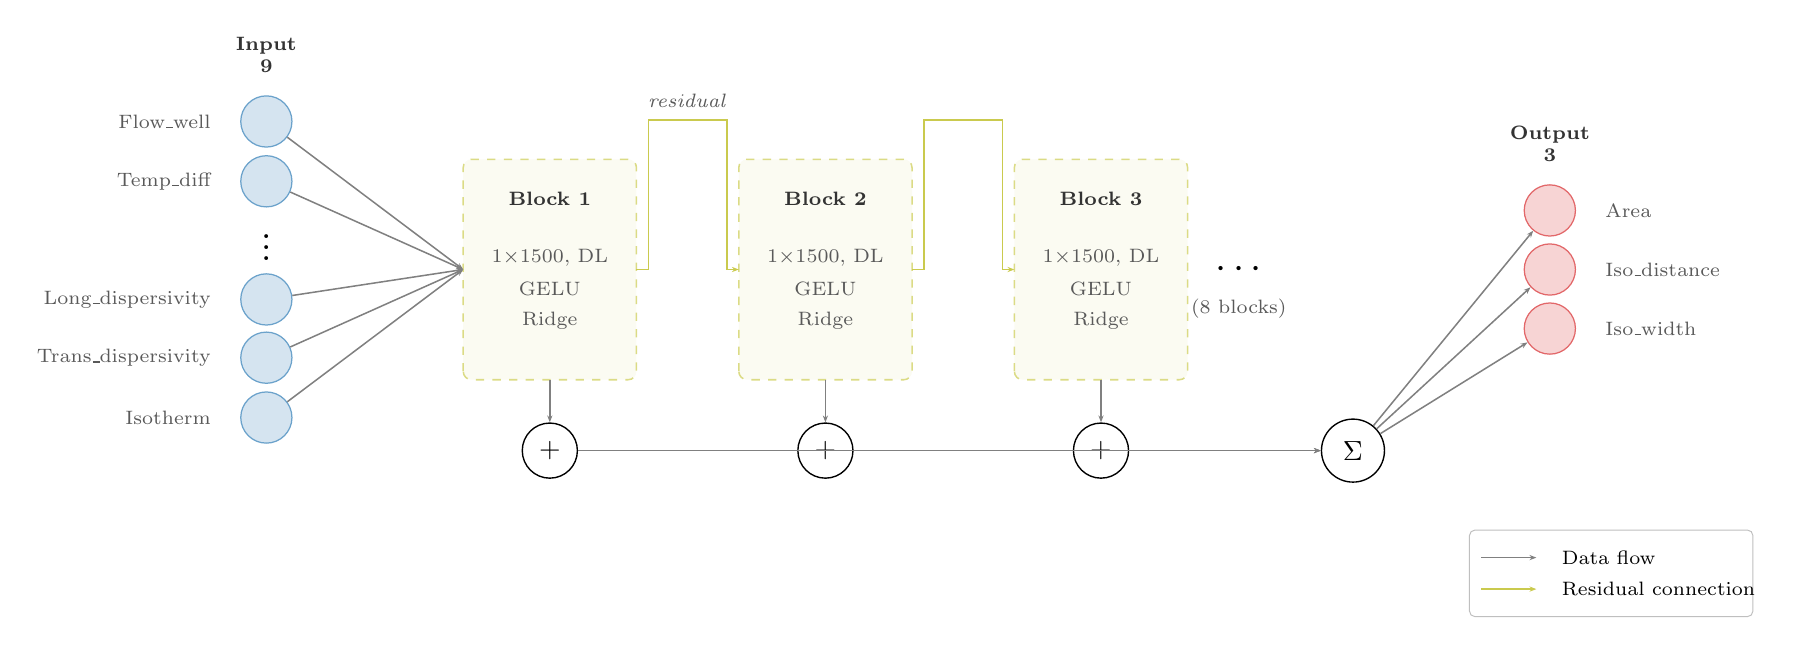
\begin{tikzpicture}
    \node[input node] (in_0) at (0.00,1.88) {};
    \node[annot, left=2.5mm of in_0] {Flow\_well};
    \node[input node] (in_1) at (0.00,1.12) {};
    \node[annot, left=2.5mm of in_1] {Temp\_diff};
    \node[dots node] (in_dots) at (0.00,0.38) {$\vdots$};
    \node[input node] (in_2) at (0.00,-0.38) {};
    \node[annot, left=2.5mm of in_2] {Long\_dispersivity};
    \node[input node] (in_3) at (0.00,-1.12) {};
    \node[annot, left=2.5mm of in_3] {Trans\_dispersivity};
    \node[input node] (in_4) at (0.00,-1.88) {};
    \node[annot, left=2.5mm of in_4] {Isotherm};
    \node[lbl, above=5mm] at (0.00,1.88) {Input\\9};
    \draw[resbox] (2.50,-1.4) rectangle (4.70,1.4);
    \node[lbl] at (3.60,0.90) {Block 1};
    \node[annot] at (3.60,0.15) {1$\times$1500, DL};
    \node[annot] at (3.60,-0.25) {GELU};
    \node[annot] at (3.60,-0.65) {Ridge};
    \node[sum node] (sum0) at (3.60,-2.30) {$+$};
    \draw[arr] (3.60,-1.4) -- (sum0);
    \draw[resbox] (6.00,-1.4) rectangle (8.20,1.4);
    \node[lbl] at (7.10,0.90) {Block 2};
    \node[annot] at (7.10,0.15) {1$\times$1500, DL};
    \node[annot] at (7.10,-0.25) {GELU};
    \node[annot] at (7.10,-0.65) {Ridge};
    \node[sum node] (sum1) at (7.10,-2.30) {$+$};
    \draw[arr] (7.10,-1.4) -- (sum1);
    \draw[resbox] (9.50,-1.4) rectangle (11.70,1.4);
    \node[lbl] at (10.60,0.90) {Block 3};
    \node[annot] at (10.60,0.15) {1$\times$1500, DL};
    \node[annot] at (10.60,-0.25) {GELU};
    \node[annot] at (10.60,-0.65) {Ridge};
    \node[sum node] (sum2) at (10.60,-2.30) {$+$};
    \draw[arr] (10.60,-1.4) -- (sum2);
    \node[font=\Large] at (12.35,0) {$\cdots$};
    \node[annot] at (12.35,-0.5) {(8 blocks)};

    % input to block 1
    \draw[arr] (in_0) -- (2.50,0);
    \draw[arr] (in_1) -- (2.50,0);
    \draw[arr] (in_2) -- (2.50,0);
    \draw[arr] (in_3) -- (2.50,0);
    \draw[arr] (in_4) -- (2.50,0);

    % residual flow
    \draw[-{Stealth[length=2.5pt]}, residualcol!80, line width=0.5pt] (4.70,0) -- ++(0.15,0) |- (4.85,1.90) -- (5.85,1.90) |- (6.00,0);
    \draw[-{Stealth[length=2.5pt]}, residualcol!80, line width=0.5pt] (8.20,0) -- ++(0.15,0) |- (8.35,1.90) -- (9.35,1.90) |- (9.50,0);
    \node[annot, above=1pt] at (5.35,1.90) {\textit{residual}};
    \node[sum node, minimum size=8mm] (sigma) at (13.80,-2.30) {$\Sigma$};
    \draw[arr] (sum0) -- (sigma);
    \draw[arr] (sum1) -- (sigma);
    \draw[arr] (sum2) -- (sigma);
    \node[output node] (out_0) at (16.30,0.75) {};
    \node[annot, right=2.5mm of out_0] {Area};
    \node[output node] (out_1) at (16.30,0.00) {};
    \node[annot, right=2.5mm of out_1] {Iso\_distance};
    \node[output node] (out_2) at (16.30,-0.75) {};
    \node[annot, right=2.5mm of out_2] {Iso\_width};
    \node[lbl, above=5mm] at (16.30,0.75) {Output\\3};
    \draw[arr] (sigma) -- (out_0);
    \draw[arr] (sigma) -- (out_1);
    \draw[arr] (sigma) -- (out_2);

    % legend
    \begin{scope}[shift={($(current bounding box.south east)+(0.3,-0.6)$)}]
    \fill[white, rounded corners=2pt, draw=black!25, line width=0.35pt] (0,0) rectangle (-3.6,-1.10);
    \draw[arr] (-3.45,-0.35) -- (-2.75,-0.35);
    \node[anchor=west, font=\scriptsize] at (-2.55,-0.35) {Data flow};
    \draw[-{Stealth[length=2.5pt]}, residualcol!80, line width=0.5pt] (-3.45,-0.75) -- (-2.75,-0.75);
    \node[anchor=west, font=\scriptsize] at (-2.55,-0.75) {Residual connection};
    \end{scope}

    % title
%     \node[font=\bfseries, above=8mm] at (current bounding box.north) {SResdRVFL (Isotherm)};
\end{tikzpicture}
\end{document}
